\documentclass[semifinal]{cpecmu}

%% This is a sample document demonstrating how to use the CPECMU
%% project template. If you are having trouble, see "cpecmu.pdf" for
%% documentation.

\projectNo{S002-2}
\acadyear{2024}

\titleTH{เว็บไซต์ระบบสังคมสงเคราะห์}
\titleEN{Welfare Web System}

\author{นายกิตปกรณ์ ทองโคตร}{Kitpakorn Thongkot}{650610749}
\author{นายนรภัทร จินดาสุ่น}{Norapat Chindasoon}{650610774}
\author{นายปัณณวิชญ์ เศรษฐสิริวาณิช}{Pannawit Setsiriwanit}{650610784}

\cpeadvisor{dome}
\cpecommittee{lachana}
\cpecommittee{nasi}
% \committee{ผศ.ดร.\,ลัชนา ระมิงค์วงศ์}{Asst.\,Prof.\,Dr.\,Lachana Ramingwong, Ph.D.}

%% Some possible packages to include:
\usepackage[final]{graphicx} % for including graphics

%% Add bookmarks and hyperlinks in the document.
\PassOptionsToPackage{hyphens}{url}
\usepackage[colorlinks=true,allcolors=Blue4,citecolor=red,linktoc=all]{hyperref}
\def\UrlLeft#1\UrlRight{$#1$}

%% Needed just by this example, but maybe not by most reports
\usepackage{afterpage} % for outputting
\usepackage{pdflscape} % for landscape figures and tables. 
\usepackage{float}
%% Some other useful packages. Look these up to find out how to use
%% them.
% \usepackage{natbib}    % for author-year citation styles
% \usepackage{txfonts}
% \usepackage{appendix}  % for appendices on a per-chapter basis
% \usepackage{xtab}      % for tables that go over multiple pages
% \usepackage{subfigure} % for subfigures within a figure
% \usepackage{pstricks,pdftricks} % for access to special PostScript and PDF commands
% \usepackage{nomencl}   % if you have a list of abbreviations

%% if you're having problems with overfull boxes, you may need to increase
%% the tolerance to 9999
% \tolerance=9999

\bibliographystyle{plain}
% \bibliographystyle{IEEEbib}

% \renewcommand{\topfraction}{0.85}
% \renewcommand{\textfraction}{0.1}
% \renewcommand{\floatpagefraction}{0.75}

%% Example for glossary entry
%% Need to use glossary option
%% See glossaries package for complete documentation.
\ifglossary
  \newglossaryentry{lorem ipsum}{
    name=lorem ipsum,
    description={derived from Latin dolorem ipsum, translated as ``pain itself''}
  }
\fi

%% Uncomment this command to preview only specified LaTeX file(s)
%% imported with \include command below.
%% Any other file imported via \include but not specified here will not
%% be previewed.
%% Useful if your report is large, as you might not want to build
%% the entire file when editing a certain part of your report.
% \includeonly{chapters/intro,chapters/background}

\begin{document}
\maketitle
\makesignature

\ifproject
\begin{abstractTH}

โครงการนี้มีวัตถุประสงค์เพื่อพัฒนา ระบบจัดเก็บข้อมูลสำหรับนักสังคมสงเคราะห์ ประจำโรงพยาบาลมหาราชนครเชียงใหม่ เนื่องจากปัจจุบันยังไม่มีระบบที่มีประสิทธิภาพในการจัดการข้อมูล ส่งผลให้กระบวนการทำงานอาจเกิดความล่าช้าและส่งผลต่อการให้บริการแก่ผู้รับสวัสดิการ

ระบบที่พัฒนาขึ้นเป็น เว็บแอปพลิเคชัน ที่ช่วยให้นักสังคมสงเคราะห์สามารถจัดเก็บและบริหารจัดการข้อมูลได้อย่างเป็นระบบ ทั้งยังสามารถนำข้อมูลที่บันทึกไว้มาวิเคราะห์และต่อยอดการทำงานได้อย่างสะดวกและมีประสิทธิภาพยิ่งขึ้น

เว็บแอปพลิเคชันดังกล่าวพัฒนาด้วย Next.js สำหรับฝั่ง Front-end และใช้ NestJS สำหรับ Back-end ในส่วนของฐานข้อมูล ใช้ PostgreSQL เพื่อจัดเก็บและบริหารจัดการข้อมูลอย่างเป็นระบบ นอกจากนี้ การทดสอบและการปรับใช้ (Deployment) ระบบจะดำเนินการผ่าน Docker เพื่อความยืดหยุ่นและประสิทธิภาพสูงสุดในการใช้งาน
\end{abstractTH}

\begin{abstract}

This project aims to develop a data management system for social workers at Maharaj Nakorn Chiang Mai Hospital. Currently, there is no efficient system for managing information, which may cause delays in work processes and affect the delivery of services to beneficiaries.

The developed system is a web application designed to help social workers systematically store and manage data. Additionally, it enables users to analyze and utilize stored information to enhance their work efficiency.
    
The web application is built using Next.js for the front-end and NestJS for the back-end. For database management, PostgreSQL is used to store and organize data effectively. Furthermore, the system's testing and deployment are carried out using Docker to ensure flexibility and optimal performance.
\end{abstract}

\iffalse
\begin{dedication}
This document is dedicated to all Chiang Mai University students.

Dedication page is optional.
\end{dedication}
\fi % \iffalse

\begin{acknowledgments}

โครงงานนี้จะไม่สามารถสำเร็จลุล่วงไปได้ หากไม่ได้รับความอนุเคราะห์และการสนับสนุนจากหลายฝ่าย ข้าพเจ้าขอแสดงความขอบคุณเป็นอย่างยิ่งต่อ ผศ.โดม โพธิกานนท์ อาจารย์ที่ปรึกษาโครงงาน ที่สละเวลาอันมีค่าให้คำแนะนำ ให้แนวคิด และชี้แนะแหล่งความรู้ที่จำเป็นสำหรับการพัฒนาเว็บแอปพลิเคชัน ตลอดจนช่วยตรวจสอบและแก้ไขข้อบกพร่องต่าง ๆ ด้วยความเอาใจใส่มาโดยตลอด

นอกจากนี้ ข้าพเจ้าขอขอบพระคุณ ผศ.ดร.ลัชนา ระมิงค์วงศ์ และ อ.ดร.นษิ ตันติธารานุกุล ที่ให้คำปรึกษาและข้อเสนอแนะอันเป็นประโยชน์ จนทำให้โครงงานนี้มีความสมบูรณ์ยิ่งขึ้น

ขอขอบคุณเพื่อนๆ และรุ่นพี่ทุกท่าน ที่คอยให้คำแนะนำ ให้กำลังใจ และเป็นแรงสนับสนุนตลอดมา ซึ่งเป็นพลังผลักดันสำคัญที่ทำให้ข้าพเจ้ามุ่งมั่นและตั้งใจทำงานจนสามารถพัฒนาโครงงานนี้จนสำเร็จ

สุดท้ายนี้ ข้าพเจ้าขอขอบพระคุณทุกท่านที่ไม่ได้เอ่ยนาม ณ ที่นี้ ซึ่งได้ให้ความช่วยเหลือและสนับสนุนโครงงานในรูปแบบต่างๆ ตลอดระยะเวลาการดำเนินงาน ขอบพระคุณเป็นอย่างสูง

\acksign{2025}{3}{5}
\end{acknowledgments}%
\fi % \ifproject

\contentspage

\ifproject
\figurelistpage

\tablelistpage
\fi % \ifproject

% \abbrlist % this page is optional

% \symlist % this page is optional

% \preface % this section is optional


\pagestyle{empty}\cleardoublepage
\normalspacing \setcounter{page}{1} \pagenumbering{arabic} \pagestyle{cpecmu}

\chapter{\ifenglish Introduction\else บทนำ\fi}

\section{\ifenglish Project rationale\else ที่มาของโครงงาน\fi}

ปัจจุบัน นักสังคมสงเคราะห์ที่ปฏิบัติงาน ณ โรงพยาบาลมหาราชนครเชียงใหม่ ยังคงใช้วิธีการจัดเก็บข้อมูลในรูปแบบกระดาษ ก่อนจะทำการบันทึกข้อมูลลงในคอมพิวเตอร์ของตนเองในรูปแบบไฟล์ .docx (Microsoft Word) อย่างไรก็ตาม คอมพิวเตอร์แต่ละเครื่องไม่สามารถเข้าถึงไฟล์ของกันและกันได้โดยตรง หากนักสังคมสงเคราะห์ต้องการเข้าถึงข้อมูลของผู้ใช้บริการที่ไม่ได้จัดเก็บอยู่ในคอมพิวเตอร์ของตนเอง พวกเขาจำเป็นต้องสอบถามเพื่อนร่วมงานเพื่อระบุว่าไฟล์ดังกล่าวถูกจัดเก็บอยู่ในเครื่องใด
นอกจากนี้ สำหรับข้อมูลสถิติของผู้รับบริการ นักสังคมสงเคราะห์จะบันทึกข้อมูลลงในไฟล์ .xlsx (Microsoft Excel) ซึ่งสามารถแชร์ร่วมกันระหว่างคอมพิวเตอร์หลายเครื่องได้ อย่างไรก็ตาม การจัดเก็บข้อมูลดังกล่าวดำเนินการในไฟล์เดียว โดยมีจำนวนข้อมูลสะสมหลายพันบรรทัด ส่งผลให้การสรุปผลข้อมูลในระดับรายวันหรือรายเดือนทำได้ยาก และอาจส่งผลต่อประสิทธิภาพในการบริหารจัดการข้อมูลโดยรวม

จากปัญหาที่กล่าวมาข้างต้น คณะผู้จัดทำโครงงานได้ตระหนักถึงข้อจำกัดในการจัดเก็บและบริหารจัดการข้อมูลของนักสังคมสงเคราะห์ จึงมีแนวคิดในการพัฒนา เว็บแอปพลิเคชัน เพื่อช่วยให้กระบวนการจัดการข้อมูลมีประสิทธิภาพมากยิ่งขึ้น ระบบดังกล่าวได้รับการออกแบบมาเพื่อแก้ไขปัญหาด้านการค้นหาข้อมูลให้สะดวกและรวดเร็วขึ้น รวมถึงปรับปรุงกระบวนการสรุปผลข้อมูลให้สามารถดำเนินการได้อย่างเป็นระบบและมีประสิทธิภาพยิ่งขึ้น

\section{\ifenglish Objectives\else วัตถุประสงค์ของโครงงาน\fi}
\begin{enumerate}
    \item เพื่อพัฒนาเว็บแอปพลิเคชันที่สามารถจัดเก็บข้อมูล และเข้าถึงข้อมูลได้อย่างสะดวก รวดเร็ว และมีประสิทธิภาพ
    \item เพื่อพัฒนาเว็บแอปพลิเคชันที่สามารถสรุปผลข้อมูลที่ผู้ใช้ต้องการได้ โดยไม่ต้องใช้โปรแกรมอื่นเพิ่มเติม
\end{enumerate}

\section{\ifenglish Project scope\else ขอบเขตของโครงงาน\fi}

\subsection{\ifenglish Hardware scope\else ขอบเขตด้านฮาร์ดแวร์\fi}
โครงงานนี้เป็นการพัฒนาเว็บแอปพลิเคชันที่สามารถใช้งานได้บนคอมพิวเตอร์ที่ใช้ระบบปฏิบัติการ macOS
หรือ Windows และบนโทรศัพท์มือถือที่ใช้ระบบปฏิบัติการ iOS หรือ Android
\subsection{\ifenglish Software scope\else ขอบเขตด้านซอฟต์แวร์\fi}
\begin{enumerate}
    \item เว็บแอปพลิเคชันที่สามารถเข้าใช้งานได้เฉพาะ CMU Account ที่กำหนดไว้เท่านั้น
    \item เว็บแอปพลิเคชันที่สามารถเก็บข้อมูลไฟล์ต่างๆ ได้
\end{enumerate}
\section{\ifenglish Expected outcomes\else ประโยชน์ที่ได้รับ\fi}
\begin{enumerate}
    \item ผู้ใช้สามารถจัดเก็บข้อมูลได้อย่างมีประสิทธิภาพ
    \item ผู้ใช้สามารถเข้าถึงข้อมูลได้อย่างสะดวก รวดเร็ว
    \item ผู้ใช้สามารถนำข้อมูลมาสรุปผลตามเวลาที่เลือกได้
\end{enumerate}
\section{\ifenglish Technology and tools\else เทคโนโลยีและเครื่องมือที่ใช้\fi}
\begin{itemize}
    \item ภาษาโปรแกรมมิ่ง: Typescript
    \item Front-end: Next.js, React, Tailwind CSS
    \item Back-end: NestJs, Prisma
    \item ฐานข้อมูล: PostgreSQL
    \item Object Storage: MinIO
    \item เทคโนโลยีและเครื่องมืออื่นๆ: Docker, Figma, Github
\end{itemize}    
% \subsection{\ifenglish Hardware technology\else เทคโนโลยีด้านฮาร์ดแวร์\fi}

% \subsection{\ifenglish Software technology\else เทคโนโลยีด้านซอฟต์แวร์\fi}

\section{\ifenglish Project plan\else แผนการดำเนินงาน\fi}

\begin{plan}{1}{2025}{4}{2026}
    \planitem{1}{2025}{2}{2025}{Tools Research}
    \planitem{1}{2025}{3}{2025}{Requirements}
    \planitem{5}{2025}{7}{2025}{Design}
    \planitem{7}{2025}{7}{2025}{Set up Environments}
    \planitem{8}{2025}{10}{2025}{Sprint 1: ทำระบบจัดเก็บข้อมูล}
    \planitem{11}{2025}{1}{2026}{Sprint 2: ทำระบบ login}
    \planitem{2}{2026}{4}{2026}{Sprint 3: ทำระบบสรุปข้อมูล}
    \planitem{3}{2026}{4}{2026}{Report}
\end{plan}

\newpage

\section{\ifenglish Roles and responsibilities\else บทบาทและความรับผิดชอบ\fi}
\begin{enumerate}
\item นายกิตปกรณ์ ทองโคตร รับหน้าที่ในการทำ Components ของ Front-end, Initialize Project โดยใช้ Github, วางโครงสร้างของระบบ ทั้ง Front-end และ Back-end
\item นายนรภัทร จินดาสุ่น รับหน้าที่ในการนัดหมายเพื่อพูดคุยกับ Stakeholder, ออกแบบระบบโดยใช้ Figma, จัดวางระบบ Front-end, ติดตามผลการทำงานของเพื่อนในกลุ่ม
\item นายปัณณวิชญ์ เศรษฐสิริวาณิช รับหน้าที่ในการทำระบบฐานข้อมูลทั้งหมด, ทำระบบ Back-end
\end{enumerate}

\section{\ifenglish%
Impacts of this project on society, health, safety, legal, and cultural issues
\else%
ผลกระทบด้านสังคม สุขภาพ ความปลอดภัย กฎหมาย และวัฒนธรรม
\fi}

เมื่อนักสังคมสงเคราะห์สามารถทำงานได้สะดวก รวดเร็วขึ้น ทางผู้รับบริการก็สามารถได้รับบริการได้ดีขึ้นทั้งทางตรงและทางอ้อม เช่นการบริการที่เร็วขึ้น ทำให้รับผู้รับบริการได้มากขึ้น และการสรุปผลข้อมูลก็สามารถลดภาระของนักสังคมสงเคราะห์ที่ต้องไปสรุปข้อมูลเองด้วย

\chapter{\ifenglish Background Knowledge and Theory\else ทฤษฎีที่เกี่ยวข้อง\fi}

\section{หน้าที่ของนักสังคมเคราะห์}

นักสังคมสงเคราะห์มีหน้าที่สำคัญในการช่วยเหลือและสนับสนุนบุคคล ครอบครัว และชุมชนที่เผชิญปัญหาทางสังคม อารมณ์ หรือเศรษฐกิจ เพื่อให้สามารถปรับตัวและดำเนินชีวิตในสังคมได้อย่างเหมาะสม โดยมีบทบาทที่ครอบคลุมหลายด้าน ซึ่งแต่ละบทบาทล้วนมีความสำคัญต่อคุณภาพชีวิตของผู้ที่ต้องการความช่วยเหลือ

\subsection{ให้คำปรึกษาและแนะแนวทางช่วยเหลือ}

นักสังคมสงเคราะห์ให้คำปรึกษาโดยรับฟัง ประเมินปัญหา และให้แนวทางแก้ไข พร้อมแนะนำสิทธิและสวัสดิการที่เหมาะสม เพื่อให้ผู้ที่ต้องการความช่วยเหลือได้รับการดูแลอย่างเหมาะสม
\subsection{ประสานงานและส่งต่อหน่วยงานที่เกี่ยวข้อง}

นักสังคมสงเคราะห์ทำงานร่วมกับบุคลากรด้านสุขภาพและสวัสดิการเพื่อให้ผู้ป่วยได้รับการดูแลครบถ้วน พวกเขาประสานงานกับหน่วยงานต่าง ๆ เพื่อจัดหาความช่วยเหลือเพิ่มเติม เช่น ที่พักพิง การสนับสนุนทางกฎหมาย และการเข้าถึงบริการทางสังคม

\subsection{ช่วยเหลือกลุ่มเปราะบางในสังคม}

นักสังคมสงเคราะห์ช่วยเหลือกลุ่มเปราะบาง เช่น เด็กถูกทอดทิ้ง ผู้สูงอายุไร้ผู้ดูแล ผู้พิการ และคนไร้บ้าน โดยจัดหาทรัพยากรที่จำเป็น เช่น อาหาร ที่พัก และเงินสนับสนุน พร้อมให้ความรู้เพื่อพัฒนาคุณภาพชีวิตและส่งเสริมการพึ่งพาตนเอง
\subsection{ติดตามผลและประเมินสถานการณ์}

นักสังคมสงเคราะห์ติดตามผลการช่วยเหลืออย่างต่อเนื่อง เพื่อให้แน่ใจว่าตรงกับความต้องการของแต่ละบุคคล หากพบปัญหาเพิ่มเติม พวกเขาจะปรับแผนให้เหมาะสม พร้อมจัดทำรายงานเพื่อใช้พัฒนาระบบสวัสดิการในอนาคต

\newpage
\section{ด้านเทคโนโลยีที่ใช้พัฒนาเว็บแอปพลิเคชัน}
\subsection{Typescript}
TypeScript เป็นภาษาโปรแกรมที่พัฒนาโดย Microsoft ซึ่งเพิ่มระบบตรวจสอบ Type ให้กับ JavaScript ทำให้สามารถควบคุมและจัดการ Type ในโปรแกรมได้อย่างมีประสิทธิภาพ ช่วยลดข้อผิดพลาดที่อาจเกิดขึ้นก่อนรันโปรแกรม ซึ่งเป็นข้อได้เปรียบสำคัญในการพัฒนาแอปพลิเคชันขนาดใหญ่ เนื่องจากใน JavaScript ข้อผิดพลาดเกี่ยวกับ Type มักจะปรากฏขึ้นในระหว่างการทำงานของโปรแกรม \cite{aiw}

\begin{figure}[H]
  \begin{center}
  
\includegraphics[width=0.2\textwidth]{typescript_original_logo_icon_146317.png}
  \end{center}
  \caption[Typescript]{Typescript}
\end{figure}
\subsection{React}
React เป็นไลบรารี JavaScript ที่พัฒนาโดย Facebook โดยถูกออกแบบมาเพื่อช่วยในการสร้าง User Interface (UI) ที่มีประสิทธิภาพและยืดหยุ่นสูง โครงสร้างหลักของ React คือแนวคิดเกี่ยวกับ Component-Based Architecture ซึ่งช่วยให้การพัฒนา UI เป็นไปอย่างเป็นระบบ แต่ละ Component สามารถนำกลับมาใช้ซ้ำได้ React ใช้แนวคิด Virtual DOM เพื่อเพิ่มประสิทธิภาพในการอัปเดต UI โดยการเปรียบเทียบความเปลี่ยนแปลงก่อนที่จะเรนเดอร์จริง ทำให้การทำงานรวดเร็วและลดภาระของเบราว์เซอร์ React ได้รับความนิยมอย่างแพร่หลายในวงการพัฒนาเว็บแอปพลิเคชัน เนื่องจากช่วยให้การจัดการ UI ซับซ้อนทำได้ง่ายขึ้น และสามารถรองรับการพัฒนาแบบไดนามิกได้เป็นอย่างดี \cite{aiw2}
\begin{figure}[H]
  \begin{center}
  
\includegraphics[width=0.2\textwidth]{1174949_js_react js_logo_react_react native_icon.png}
  \end{center}
  \caption[React]{React}
\end{figure}

\newpage

\subsection{Next.js}
Next.js เป็น React Web Framework ที่ออกแบบมาเพื่อให้การพัฒนาเว็บแอปพลิเคชันสะดวกขึ้น โดยมีการตั้งค่าและการคอนฟิกหลายๆ อย่างให้พร้อมใช้งาน เช่น การไม่ต้องตั้งค่าใดๆ เอง (Zero Config) และสามารถใช้งานได้ทันทีในสภาพแวดล้อมการผลิต (Ready for Production) นอกจากนี้ Next.js รองรับการทำ SEO ได้ดีกว่า React ปกติ เนื่องจากเป็นการเรนเดอร์แบบ Server Side Rendering (SSR) ซึ่งแตกต่างจาก React ที่ส่วนใหญ่ใช้ Client Side Rendering ในการทำงาน นอกจากนี้ยังรองรับฟีเจอร์เช่น Code Splitting, Static Site Generation (SSG), การสร้าง Dynamic Page, การสร้าง APIs และการปรับแต่งเซิร์ฟเวอร์ได้ รวมถึงมีเอกสารประกอบที่อ่านเข้าใจง่ายและมีตัวอย่างให้ศึกษา ทำให้ผู้ที่เคยใช้งาน React สามารถเริ่มใช้งาน Next.js ได้อย่างรวดเร็วและไม่ยาก \cite{aiw3}
\begin{figure}[H]
  \begin{center}
  
\includegraphics[width=0.2\textwidth]{next-js-seeklogo.png}
  \end{center}
  \caption[Next.js]{Next.js}
\end{figure}
\subsection{Nest JS}
Nest JS เป็น Framework สำหรับพัฒนาแอปพลิเคชันฝั่งเซิร์ฟเวอร์ที่สร้างขึ้นบน Node.js โดยออกแบบมาให้มีประสิทธิภาพและยืดหยุ่นสูง โครงสร้างของ Nest JS ถูกออกแบบให้ใช้ TypeScript เป็นหลัก (แม้ว่าจะรองรับ JavaScript ด้วย) และยึดแนวคิดเชิง Object-Oriented Programming (OOP) อย่างสมบูรณ์ ซึ่งช่วยให้การจัดระเบียบโค้ดเป็นไปอย่างเป็นระบบและมีโครงสร้างที่ชัดเจน นอกจากนี้ NestJS ยังสามารถทำงานร่วมกับไลบรารีอื่นๆ ได้อย่างง่ายดาย เช่น Express.js และ Socket.io ทำให้สามารถขยายขีดความสามารถของแอปพลิเคชันได้อย่างยืดหยุ่นและมีประสิทธิภาพ \cite{aiw4}
\begin{figure}[H]
  \begin{center}
  
\includegraphics[width=0.2\textwidth]{nest-js-icon.png}
  \end{center}
  \caption[Nest JS]{Nest JS}
\end{figure}

\newpage

\subsection{PostgreSQL}
PostgreSQL เป็นระบบจัดการฐานข้อมูลเชิงสัมพันธ์แบบโอเพ่นซอร์สระดับองค์กรที่ทรงพลัง รองรับทั้งการจัดเก็บข้อมูลแบบเชิงสัมพันธ์ผ่าน SQL และข้อมูลแบบไม่เชิงสัมพันธ์ผ่าน JSON โดดเด่นด้วยความน่าเชื่อถือ ความปลอดภัย และความแม่นยำในระดับสูง อีกทั้งยังได้รับการสนับสนุนจากชุมชนผู้พัฒนาที่แข็งแกร่ง ด้วยประสิทธิภาพและความยืดหยุ่นของ PostgreSQL ทำให้เป็นตัวเลือกหลักสำหรับเว็บแอปพลิเคชัน อุปกรณ์พกพา และโซลูชันด้านการวิเคราะห์ข้อมูลเชิงพื้นที่ที่ต้องการระบบฐานข้อมูลที่มีเสถียรภาพสูง \cite{aiw6}
\begin{figure}[H]
  \begin{center}
  
\includegraphics[width=0.2\textwidth]{PostgreSQL-Logo.wine.png}
  \end{center}
  \caption[PostgreSQL]{PostgreSQL}
\end{figure}
\subsection{MinIO}
MinIO เป็นระบบจัดเก็บข้อมูลแบบ Object Storage ที่รองรับการจัดเก็บข้อมูลประเภทต่างๆ เช่น ไฟล์ไบนารี, ไฟล์เสียง, รูปภาพ, วิดีโอ และสเปรดชีต โดยผู้ใช้สามารถเข้าถึงและจัดการข้อมูลที่เก็บอยู่ใน MinIO ผ่าน REST API ทำให้สามารถเชื่อมต่อกับแอปพลิเคชันหรือระบบต่างๆ ได้อย่างสะดวกและมีประสิทธิภาพ \cite{aiw5}
\begin{figure}[H]
  \begin{center}
  
\includegraphics[width=0.2\textwidth]{cdnlogo.com_minio.png}
  \end{center}
  \caption[MinIO]{MinIO}
\end{figure}
\subsection{Docker}
Docker เป็นแพลตฟอร์มซอฟต์แวร์ที่ช่วยให้การสร้าง ทดสอบ และปรับใช้แอปพลิเคชันเป็นไปอย่างรวดเร็วและมีประสิทธิภาพ โดยใช้ คอนเทนเนอร์ (Containers) ซึ่งเป็นหน่วยบรรจุซอฟต์แวร์ที่รวมทุกองค์ประกอบที่จำเป็นสำหรับการทำงาน เช่น ไลบรารี เครื่องมือระบบ โค้ด และรันไทม์ ทำให้สามารถรันแอปพลิเคชันได้อย่างเสถียรในทุกสภาพแวดล้อม ด้วยความสามารถนี้ Docker ช่วยให้การปรับใช้และขยายขนาดแอปพลิเคชันเป็นไปอย่างราบรื่นและมั่นใจได้ว่าโค้ดจะทำงานได้อย่างสม่ำเสมอในทุกระบบ \cite{aiw7}
\begin{figure}[H]
  \begin{center}
  
\includegraphics[width=0.2\textwidth]{4373190_docker_logo_logos_icon.png}
  \end{center}
  \caption[Docker]{Docker}
\end{figure}
\subsection{Tailwind CSS}
Tailwind CSS เป็นหนึ่งใน CSS Framework ที่ออกแบบมาในแนวทาง Utility-first ซึ่งหมายความว่าแต่ละคลาสใน Tailwind จะกำหนดคุณสมบัติของ CSS เพียงหนึ่งอย่างโดยเฉพาะ เช่น สีพื้นหลัง (background-color), ขอบ (border), ขนาดตัวอักษร (font-size) และอื่น ๆ แทนที่จะเป็นคลาสที่รวมชุดคำสั่งสำเร็จรูปไว้

Tailwind จึงเหมาะสำหรับนักพัฒนาที่ต้องการความยืดหยุ่นสูงในการออกแบบหน้าเว็บ เนื่องจากสามารถกำหนดสไตล์ขององค์ประกอบต่าง ๆ ได้อย่างแม่นยำโดยไม่ต้องพึ่งพาคลาสคอมโพเนนต์สำเร็จรูป ซึ่งมักมีข้อจำกัดในการปรับแต่ง นอกจากนี้ การใช้ Tailwind ยังช่วยให้การจัดการโค้ด CSS เป็นระบบมากขึ้น ลดความซับซ้อนของไฟล์สไตล์ชีต และส่งเสริมแนวทางการพัฒนาเว็บที่มีประสิทธิภาพ \cite{aiw8}
\begin{figure}[H]
  \begin{center}
  
\includegraphics[width=0.2\textwidth]{pngwing.com (4).png}
  \end{center}
  \caption[Tailwind CSS]{Tailwind CSS}
\end{figure}

\subsection{Prisma}
Prisma ORM เป็นเครื่องมือสำหรับจัดการฐานข้อมูลในแอปพลิเคชัน TypeScript และ JavaScript ที่ช่วยให้การทำงานกับฐานข้อมูลมีประสิทธิภาพและใช้งานง่ายขึ้น

Prisma มีเครื่องมือสำหรับ จัดการโครงสร้างฐานข้อมูล (schema management), ทำ migrations และเรียกใช้งานข้อมูลผ่าน Prisma Client ซึ่งช่วยลดความซับซ้อนของ SQL Query รองรับฐานข้อมูลยอดนิยม เช่น PostgreSQL, MySQL, SQLite และ MongoDB ทำให้เป็นตัวเลือกที่เหมาะสำหรับนักพัฒนาที่ต้องการความยืดหยุ่นในการจัดการข้อมูล \cite{aiw9}
\begin{figure}[H]
  \begin{center}
  
\includegraphics[width=0.2\textwidth]{pngwing.com (3).png}
  \end{center}
  \caption[Prisma]{Prisma}
\end{figure}

\newpage

\section{\ifenglish%
\ifcpe CPE \else ISNE \fi knowledge used, applied, or integrated in this project
\else%
ความรู้ตามหลักสูตรซึ่งถูกนำมาใช้หรือบูรณาการในโครงงาน
\fi
}
\begin{itemize}

  \item[-] \textbf{Fundamentals of Database Systems (261342)} ศึกษาหลักการออกแบบและการใช้งานฐานข้อมูล โดยใช้ MySQL ในการสร้าง เชื่อมต่อ และจัดการฐานข้อมูล รวมถึงการเขียนคำสั่ง SQL เพื่อจัดการข้อมูลภายในฐานข้อมูล
  \item[-] \textbf{Software Engineering (261361)} ศึกษากระบวนการทางวิศวกรรมซอฟต์แวร์ ตั้งแต่การเก็บรวบรวมความต้องการของผู้ใช้ การกำหนดเป้าหมายของระบบ การวางแผนการทำงาน การประเมินและทดสอบระบบ ไปจนถึงการปรับปรุงและแก้ไขระบบให้มีประสิทธิภาพ
  \item[-] \textbf{Basic CPE Lab (261207)} ฝึกปฏิบัติการพัฒนาเว็บแอปพลิเคชัน โดยประยุกต์ใช้ความรู้ด้าน HTML สำหรับการพัฒนา Front-End และ Python สำหรับการพัฒนา Back-End รวมถึงการออกแบบ UX/UI เพื่อให้ระบบใช้งานได้อย่างมีประสิทธิภาพ
  \item[-] \textbf{Selected Topics in Computer Engineering (261494)} ศึกษาและประยุกต์ใช้เทคโนโลยี Docker และ Cloud ในการสร้างระบบจำลองสำหรับพัฒนาเว็บแอปพลิเคชัน
  \item[-] \textbf{Object-Oriented Programming (261200)} ศึกษาหลักการเขียนโปรแกรมเชิงวัตถุ (OOP) และการใช้ Model-View-Controller (MVC) รวมถึงการใช้ Web socket ในการออกแบบและพัฒนาเว็บแอปพลิเคชัน

\end{itemize}

% \section{\ifenglish%
% Extracurricular knowledge used, applied, or integrated in this project
% \else%
% ความรู้นอกหลักสูตรซึ่งถูกนำมาใช้หรือบูรณาการในโครงงาน
% \fi
% }

% อธิบายถึงความรู้ต่างๆ ที่เรียนรู้ด้วยตนเอง และแนวทางการนำความรู้เหล่านั้นมาใช้ในโครงงาน

\chapter{\ifproject%
\ifenglish Project Structure and Methodology\else โครงสร้างและขั้นตอนการทำงาน\fi
\else%
\ifenglish Project Structure\else โครงสร้างของโครงงาน\fi
\fi
}

ในบทนี้จะกล่าวถึงหลักการ และการออกแบบระบบ

\makeatletter

% \renewcommand\section{\@startsection {section}{1}{\z@}%
%                                    {13.5ex \@plus -1ex \@minus -.2ex}%
%                                    {2.3ex \@plus.2ex}%
%                                    {\normalfont\large\bfseries}}

\makeatother
%\vspace{2ex}
% \titleformat{\section}{\normalfont\bfseries}{\thesection}{1em}{}
% \titlespacing*{\section}{0pt}{10ex}{0pt}

\section{โครงสร้างของระบบ}

ภาพรวมโครงสร้างของระบบ จะเป็นดังรูปนี้

\begin{figure}[H]
  \begin{center}
  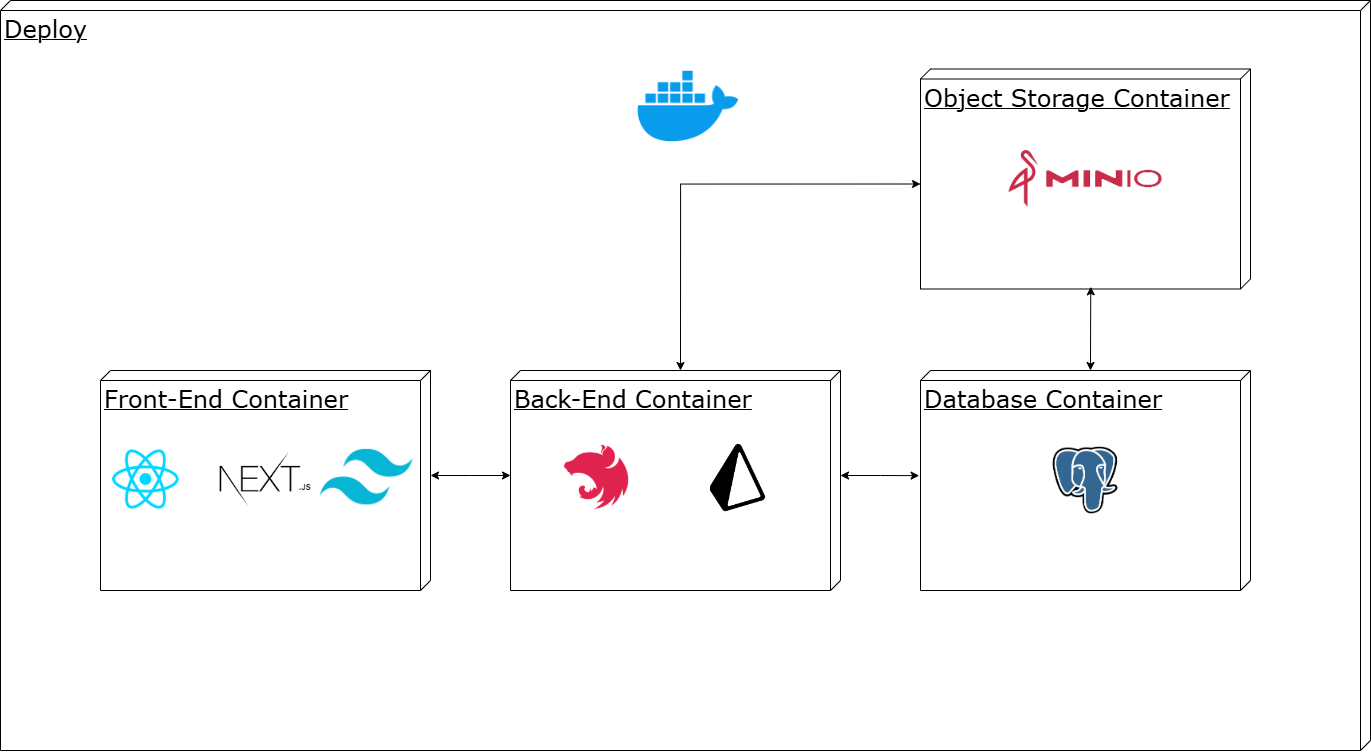
\includegraphics[width=1\textwidth]{Untitled Diagram.drawio (3).png}
  \end{center}
  \caption[โครงสร้างของระบบ]{โครงสร้างของระบบ}
\end{figure}
\subsection{Front-end}
\begin{itemize}
\item เลือกใช้ Next.js และ React เพราะมีความสำเร็จรูปในตัวเอง มีเครื่องมือที่มีให้ใช้พร้อม และยังเป็นที่ใช้แพร่หลาย ทำให้สามารถค้นหาข้อมูลเกี่ยวกับ Framework ได้ง่าย
\item เลือกใช้ Tailwind CSS เพราะเป็น component สำเร็จรูปที่สามารถ custom ได้ง่ายและเป็นที่นิยม
\end{itemize}
\subsection{Back-end}
\begin{itemize}
\item เลือกใช้ Nest JS เพราะมีความสำเร็จรูปในตัวเอง มีเครื่องมือที่พร้อมใช้งานได้เลยโดยไม่ต้องสร้างเพิ่ม 
\item เลือกใช้ MinIO เพราะเหมาะสำหรับกรณีที่ต้องการตัวเลือกการจัดเก็บข้อมูลที่มีความเร็วสูงและมีต้นทุนต่ำ สามารถใช้งานในระบบคลาวด์หรือเซิร์ฟเวอร์ขององค์กรได้ โดยไม่ต้องพึ่งพาผู้ให้บริการคลาวด์
\end{itemize}
\newpage
\subsection{Database และ Object Storage}
\begin{itemize}
\item เลือกใช้ PostgreSQL เพราะเหมาะกับข้อมูลขนาดใหญ่ ทำงานได้ดีในการอ่าน หรือ เขียน และ การวิเคราะห์ข้อมูลอย่างละเอียด 
\item เลือกใช้ Prisma เพราะมี Learning Curve ที่สูง ใช้งานง่าย และมีประสิทธิภาพดีเท่ากับตัวอื่น
\end{itemize}
\subsection{Deploy}
\begin{itemize}
\item เลือกใช้ Docker เพราะเหมาะสำหรับการรันแอปพลิเคชันที่ต้องการความยืดหยุ่นในการปรับใช้และทรัพยากรที่มีข้อจำกัด 
\end{itemize}
\newpage
\section{โครงสร้างฐานข้อมูล (Database Schema)}

ภาพรวมโครงสร้างของฐานข้อมูล จะเป็นดังรูปนี้

\begin{figure}[H]
  \begin{center}
  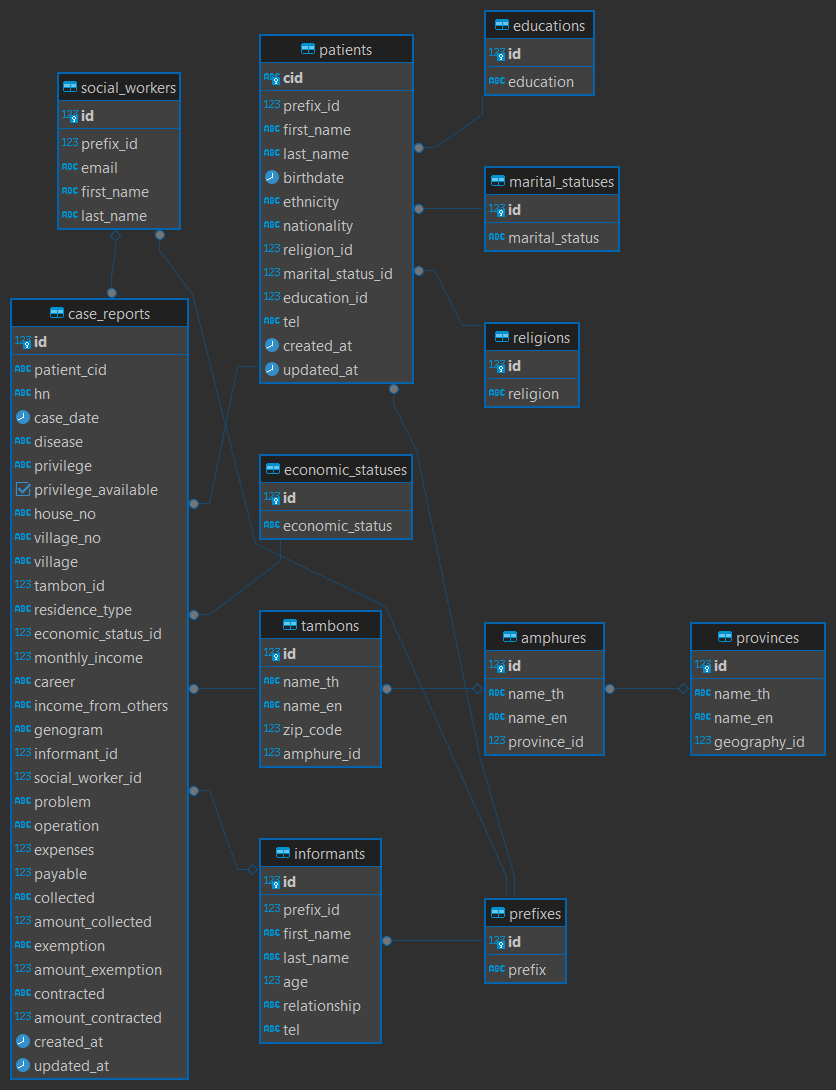
\includegraphics[width=1\textwidth]{481858458_4043514635914838_3135881775907933051_n.png}
  \end{center}
  \caption[โครงสร้างของฐานข้อมูล]{โครงสร้างของฐานข้อมูล}
\end{figure}
\newpage

\subsection{ข้อมูลผู้ป่วย}
โดยผู้ป่วย 1 คนจะมีข้อมูลได้แค่ 1 ข้อมูล
\subsection{ข้อมูลเคส}
โดยผู้ป่วย 1 คนสามารถมีได้หลายเคส (one to many)
\subsection{ข้อมูลนักสังคมสงเคราะห์}
โดยนักสังคมสงเคราะห์ 1 คนจะมีข้อมูลได้แค่ 1 ข้อมูล
\subsection{ข้อมูลผู้กรอก}
โดยเคส 1 เคสจะมีข้อมูลผู้กรอกได้แค่ 1 คนโดยอาจจะเป็นผู้ป่วยกรอกเองหรือญาติกรอกก็ได้
\subsection{ข้อมูลที่ใช้ทำ Drop-down Box}
ข้อมูลบางชนิดจะถูกเก็บไว้ในฐานข้อมูล แล้วจะถูกเรียกใช้ใน Drop-down Box เพื่อลดข้อผิดพลาดจากการพิมพ์ของนักสังคมสงเคราะห์
\begin{itemize}
\item educations
\item marital\_statuses
\item economic\_statuses
\item religions
\item prefixes
\item provinces
\item amphures
\item tambons
\end{itemize}
\chapter{\ifproject%
% \ifenglish Experimentation and Results\else การทดลองและผลลัพธ์\fi
% \else%
\ifenglish System Evaluation\else การประเมินระบบ\fi
\fi}

เนื่องจากนักสังคมสงเคราะห์ที่ปฏิบัติงานในโรงพยาบาลมหาราชนครเชียงใหม่ยังไม่มีระบบที่สามารถรองรับการทำงานได้อย่างมีประสิทธิภาพเพียงพอ หากต้องรอให้ระบบที่พัฒนาขึ้นเสร็จสมบูรณ์ อาจใช้ระยะเวลาหลายเดือน

เพื่อแก้ไขปัญหาในระยะเริ่มต้น ทางคณะผู้จัดทำโครงงานได้วางแนวทางในการให้ความช่วยเหลือเบื้องต้นแก่เจ้าหน้าที่นักสังคมสงเคราะห์ ควบคู่ไปกับการสร้างต้นแบบของแบบฟอร์มบันทึกข้อมูลเบื้องต้น เพื่อศึกษาประเด็นปัญหาที่อาจเกิดขึ้นในการพัฒนาและนำไปสู่การปรับปรุงแนวทางการทำงานใน Sprint 1 อย่างมีประสิทธิภาพ

\section{การทดลองขึ้นหน้าเว็บแอปพลิเคชัน}

โดยจะเป็นการทดลองขึ้นหน้าแบบฟอร์มกรอกประวัติผู้ป่วย ในหน้าแรกจะเป็นการกรอกข้อมูลส่วนตัวของผู้ป่วย โดยจะมีข้อมูลบางชนิดที่ต้องทำเป็น Drop-down box เพื่อลดความผิดพลาดจากการพิมพ์ของนักสังคมสงเคราะห์ และต้องกรอกให้สมบูรณ์จึงจะสามารถกรอกหน้าต่อไปได้

\begin{figure}[H]
    \begin{center}
        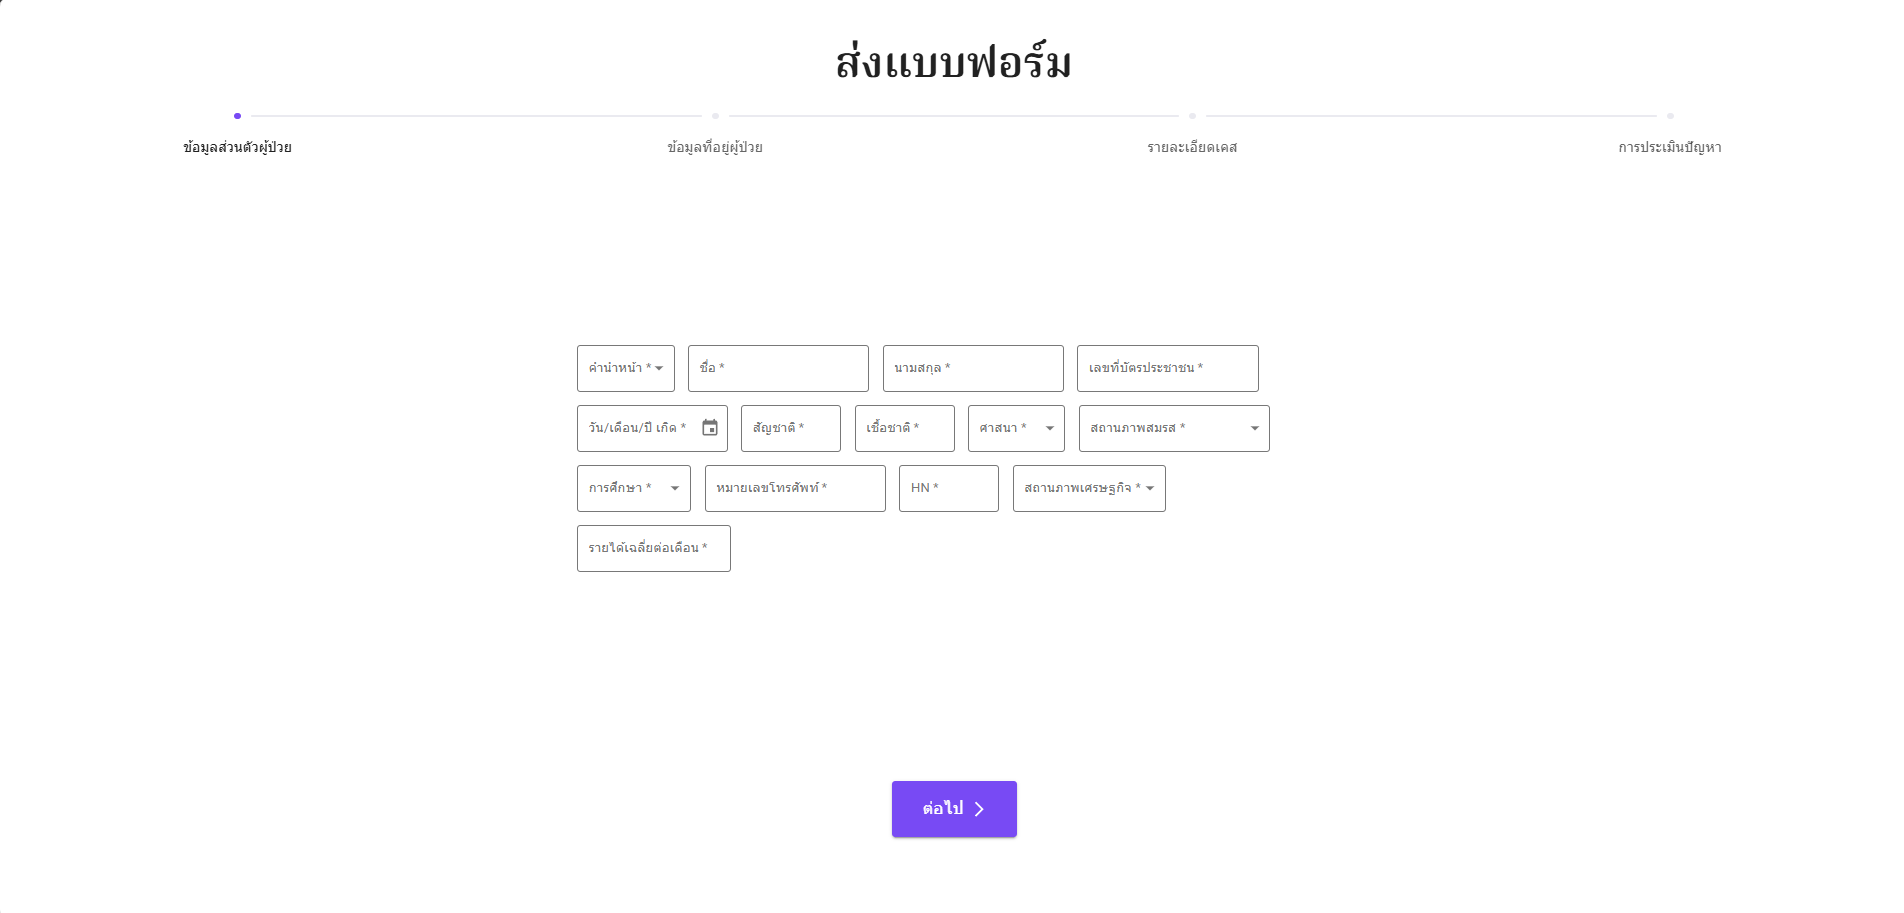
\includegraphics[width=1\textwidth]{Screenshot 2025-03-06 200233.png}
    \end{center}
    \caption[หน้ากรอกข้อมูลส่วนตัวผู้ป่วย]{หน้ากรอกข้อมูลส่วนตัวผู้ป่วย}
\end{figure}
\newpage
หน้าต่อมาคือหน้าที่ใช้กรอกที่อยู่ของผู้ป่วย ซึ่งจะสามารถกรอกได้ 2 รูปแบบ คือ
\begin{enumerate}
    \item กรอกจังหวัด อำเภอ และตำบลจากนั้นรหัสไปรษณีย์จะ Auto-complete ให้เอง
    \item กรอกแค่หมายเลขไปรษณีย์แล้ว จังหวัด อำเภอ และตำบลจะ Auto-complete ให้เอง 
\end{enumerate}
\begin{figure}[H]
    \begin{center}
        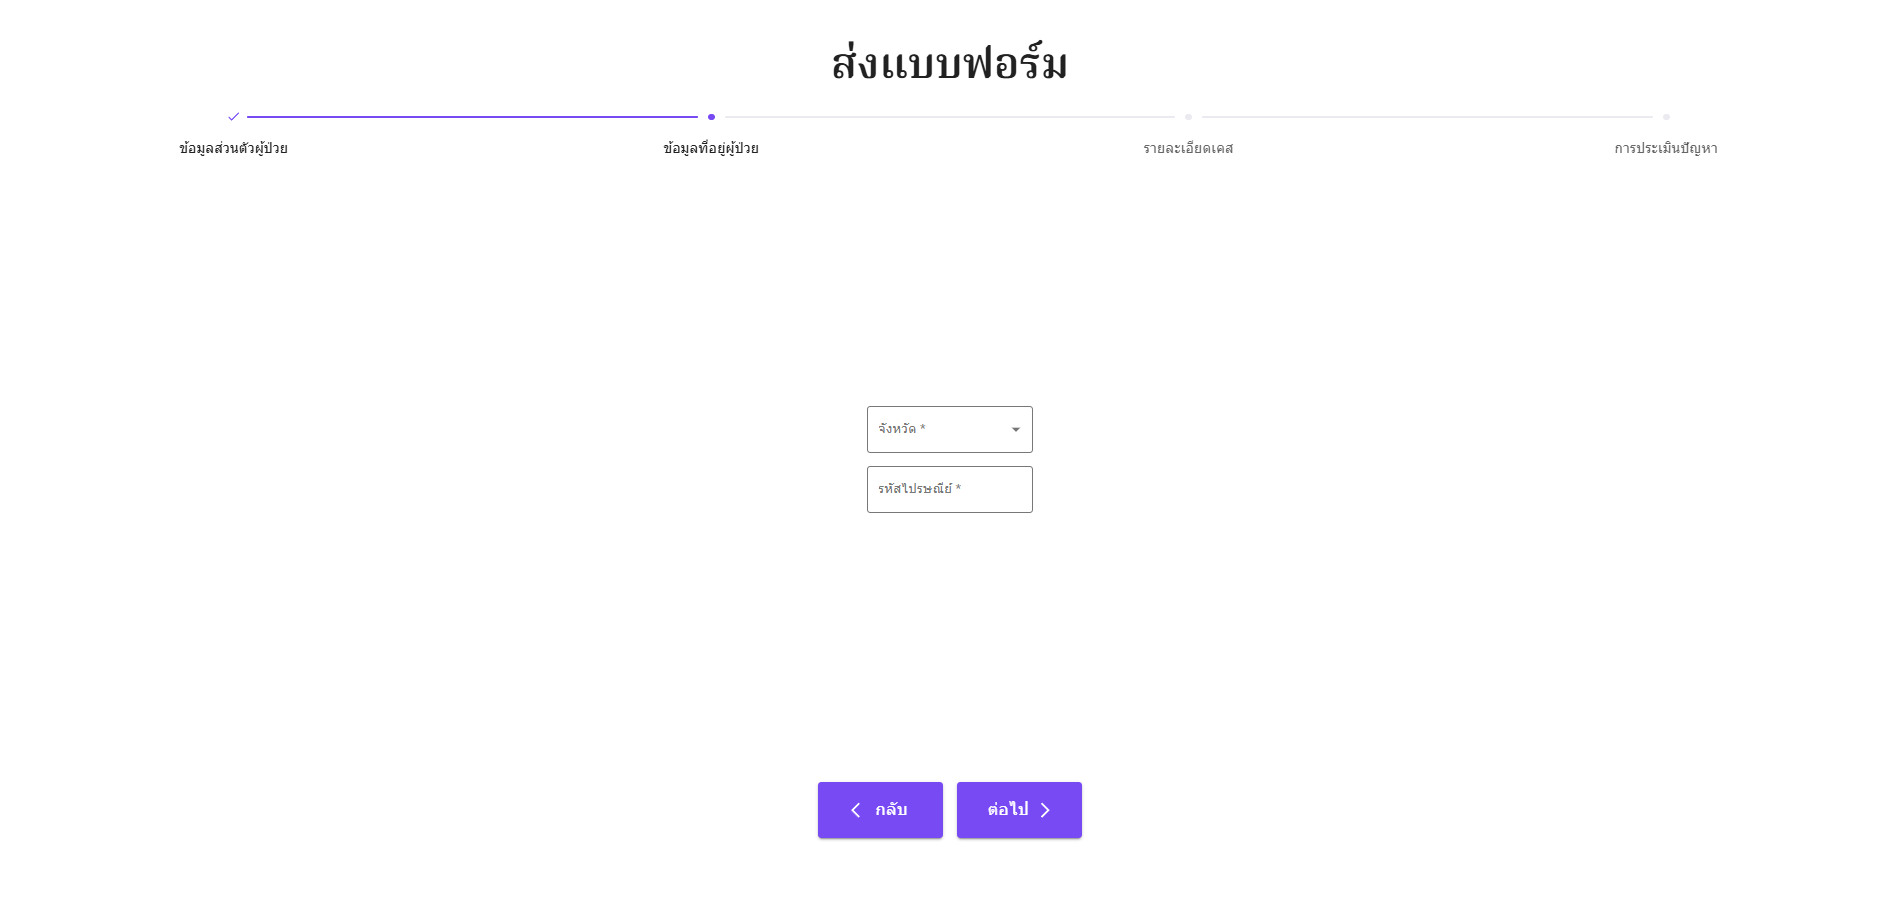
\includegraphics[width=1\textwidth]{Screenshot 2025-03-06 200323.png}
    \end{center}
    \caption[หน้ากรอกที่อยู่ผู้ป่วย]{หน้ากรอกที่อยู่ผู้ป่วย}
\end{figure}

\section{ความช่วยเหลือในเบื้องต้น}

ทางคณะผู้จัดทำโครงงาน ได้ทดลองใช้ Microsoft Form ร่วมกับ Microsoft Onedrive และ Microsoft Power Automate เพื่อให้สามารถเก็บข้อมูลและเข้าถึงข้อมูลผู้ป่วย โดยที่คอมพิวเตอร์ทุกเครื่องที่กำหนดสามารถที่จะเข้าถึงไฟล์ได้โดยตรง โดยเมื่อนักสังคมสงเคราะห์กรอกข้อมูลผู้ป่วยลงใน Mircosoft Form ทาง Microsoft Power Automate จะทำการสร้างโฟลเดอร์ของผู้ป่วยแต่ละคนใน Onedrive หากผู้ป่วยคนนั้นยังไม่มีโฟลเดอร์ของตนเอง และนำข้อมูลที่กรอกไว้ ใส่ลงในโฟลเดอร์นั้น

แต่เนื่องจาก Onedrive มีพื้นที่ที่ใช้ได้อย่างจำกัด (15 GB) ทำให้ไม่สามารถจัดเก็บข้อมูลผู้ป่วยได้อย่างเพียงพอ จึงไม่ได้นำวิธีการนี้ไปใช้จริง
\ifproject
% \include{chapters/conclusion}
\fi

\bibliography{sampleReport}

\ifproject
\normalspacing
% \appendix
% % \include{chapters/appendix}

% %% Display glossary (optional) -- need glossary option.
% \ifglossary\glossarypage\fi

% %% Display index (optional) -- need idx option.
% \ifindex\indexpage\fi

% \begin{biosketch}
% \begin{center}
%   \includegraphics[width=1.5in]{mugshot.jpg}
% \end{center}
% Your biosketch goes here. Make sure it sits inside
% the \texttt{biosketch} environment.
% \end{biosketch}
\fi % \ifproject
\end{document}
